\documentclass[
    paper=a4,
    % fontsize=12,
    % DIV=calc,
]{scrartcl}

\usepackage[T1]{fontenc}	
\usepackage[utf8]{inputenc}
\usepackage[ngerman]{babel}
\usepackage{microtype}
\usepackage{libertine}
\usepackage[libertine]{newtxmath} 

\usepackage{xcolor}
\usepackage{booktabs}
\usepackage{graphicx}
\usepackage{subcaption}
\usepackage{pdfpages}
\usepackage{svg}
\usepackage[
    locale		=	DE, 					%	Deutsche Normen
	detect-all,								%	Richtige Font im Textmodus/Mathemodus
	per-mode	=	fraction,				%	Bruchstrich darstellen
	range-units	=	repeat,					%	Einheiten wiederholt darstellen bei sirange
	range-phrase=	{{ bis }},	
]{siunitx}
\usepackage{amsmath}
\usepackage{circuitikz}


\usepackage{hyperref}

\definecolor{colorblue}{HTML}{0480CC}				% color for weblinks
\definecolor{colordarkblue}{HTML}{4C1DCC}			% no use case at the moment
\definecolor{colorgreen}{HTML}{26CC1B}				% color for missing macro
\definecolor{colorred}{HTML}{CC1204}				% color for edit macro


\KOMAoptions{
    numbers=noendperiod,
}

\hypersetup{
    bookmarksnumbered   =   true,
    breaklinks          =   true,
    colorlinks          =   true,
    linkcolor           =   colorred,
    urlcolor            =   colorblue,
    pdftitle            =   {Labor 4 Jan Hoegen},
    pdfsubject          =   {Versuchsvorbereitung Labor Digitaltechnik},    
    pdfauthor           =   {Jan Hoegen},
}

\ctikzset{
    logic ports=european,
    logic ports/scale=1.0,
    logic ports/fill=lightgray,
    tripoles/european not symbol=ieee circle,
}
\usetikzlibrary{babel}

\graphicspath{/Anhang}

\newcommand{\shadowsection}[1]{%
	\refstepcounter{section}
	\addcontentsline{toc}{section}{\protect\numberline{\thesection}{#1}}
}

\newcommand{\legend}[1]{\par\footnotesize\textbf{Legende}: #1\par}
\newcommand{\figsource}[1]{\par\footnotesize\textbf{Quelle:} #1\par}

\newcommand{\quoteenv}[1]{\glqq #1\grqq} 

\titlehead{
    \textsc{Hochschule Karlsruhe}\\
    University of Applied Sciences\\
    Studiengang EITB SS 22}
\subject{Digitaltechnik Labor 4}
\title{Parkplatzzähler: Endlich endliche Automaten}
\subtitle{Vorbereitung}
\author{Jan Hoegen\thanks{Matrikelnumer: 82358}}
\publishers{Betreuer: Prof. Dr.\,-Ing. Jan Bauer}
\date{Erstellt am: \today}


\begin{document}

\maketitle

\tableofcontents

\newpage

\section{Analyse der Parkplatzschaltung}
    Die Widerstände an den Tastern Count down und Count up sorgen dafür, dass zu jeder Zeit eine Spannung kleiner als \(V_{CC}\) an den Eingängen UP und DOWN des 74HC192 anliegt. Wird der Taster betätigt, so wird der entsprechende Eingang zwecklos geschalten und die Spannung \(V_{CC}\) fällt vollständig am Widerstand ab. In diesem Fall liegt keine Spannung mehr am Eingang an.

    Die beiden 74HC4511 sind ein BCD-zu-7-Segment-Codewandler. Abhängig der Eingangsvariablen A bis D werden die Ausgänge a bis g auf HIGH bzw. LOW gesetzt, sodass die 7 Segmente der Anzeige eine Dezimalzahl 0 bis 9 anzeigen. Dabei beschreibt das Datenblatt eine feste Codiertabelle, in der jedem Eingangszustand eine Ziffer zugeordnet wird.

    Der 74HC192 addiert jedes Mal, wenn der UP-Eingang eine positive Taktflanke aufweist, zu seinem Aktuellen Zustand die Binärzahl 0001 dazu und speichert das Ergebnis als seinen neuen Zustand. Ähnlich verhält es sich mit dem DOWN-Eingang, jedoch wird hier mit der Binärzahl 0001 subtrahiert. Dabei können die Ausgangsvariablen \(Q_0\) bis \(Q_3\) Binärzahlen von 0000 bis 1001 anzeigen. Dies entspricht den Dezimalzahlen 0 bis 9.\footnote{Der BCD-Codewandler ist ebenfalls für die Zahlen 0 bis 9 definiert, also den Binärzahlen 0000 bis 1001.} Führt das Ergebnis der beiden Summanden zu einer Zahl, die größer als dieser Zahlenbereich ist, so wird der Carry-Ausgang auf HIGH gesetzt und die Ausgänge \(Q_0\) bis \(Q_3\) auf LOW. Erzeugt die Rechnung jedoch einen Underflow, so wird borrow auf HIGH gesetzt.

    Auf die übrigen Pins des IC wird an dieser Stelle nicht näher eingegangen.

    Der erste 74HC192 führt diese Funktion genau dann aus, wenn der Taster Count up bzw. Count down nach vorherigem Drücken wieder losgelassen wird.
    Der zweite 74HC192 erhält sein Eingangssignal UP, wenn das Ergebnis des Ersten größer als 1001 ist, bzw für den Eingang DOWN bei einem Underflow.

\section{Analyse des endlichen Automaten}
    Das Zustandsdiagramm zeigt einen Moore-Automaten. Denn die Ausgangsvariablen sind lediglich vom Speicherzustand abhängig, nicht auf direkte Weise mit den Eingangsvariablen. 

    Es werden zwei D-Flip-Flops benötigt, um die Zustände zu realisieren.

\section{Auswahl der Zustandscodierung}
    Da das Ergebnis der Aufgabe 0 der dritten Laborvorbereitung \(P_T=0\) lautete, ist die Zustandscodierung aus Tabelle \ref{tab:1} zu verwenden.

    \begin{table}
        \centering
        \caption{Zustandscodierung der FSM}
        \label{tab:1}
        \begin{tabular}{ccc}\toprule
            Zustand &   $Q_1$   &   $Q_0$\\\midrule
            idle    &   0       &   0\\
            forw    &   o       &   1\\
            back    &   1       &   0\\
            wait    &   1       &   1\\\bottomrule
        \end{tabular}
    \end{table}

\section{Aufbau der Zustandsübergangstabelle}
    Nun wird die Zustandsübergangstabelle in Tabelle \ref{tab:2} vervollständigt. 

    \begin{table}
        \centering
        \caption{Zustandsübergangstabelle}
        \label{tab:2}
        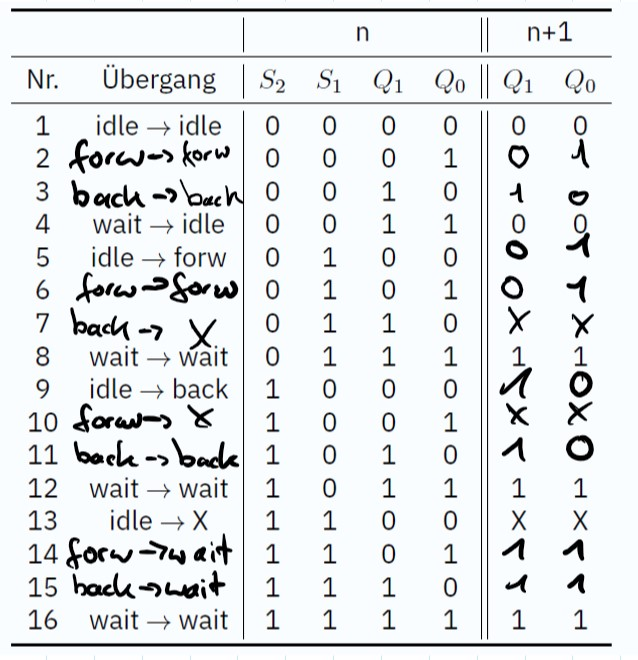
\includegraphics[width=0.7\textwidth]{Zustandsuebergang}
    \end{table}

\section{Auswahl des Standardbausteins}
    Da das Ergebnis der Aufgabe 0 der dritten Laborvorbereitung \(P_M=0\) lautete, ist das ASN und das ÜSN in Full-NAND zu realisieren.

\section{Realisierung des Übergangschaltnetzes}
    Das Übergangsschaltnetz wird mit Hilfe der Tabelle \ref{tab:2} in Full-NAND erstellt. Es gilt \(Q_0=D_0\) und \(Q_1=D_1\).
    
    \begin{minipage}{0.5\textwidth}
        \centering
            \captionof{table}{KV-Tafel für \(D_0\)}
            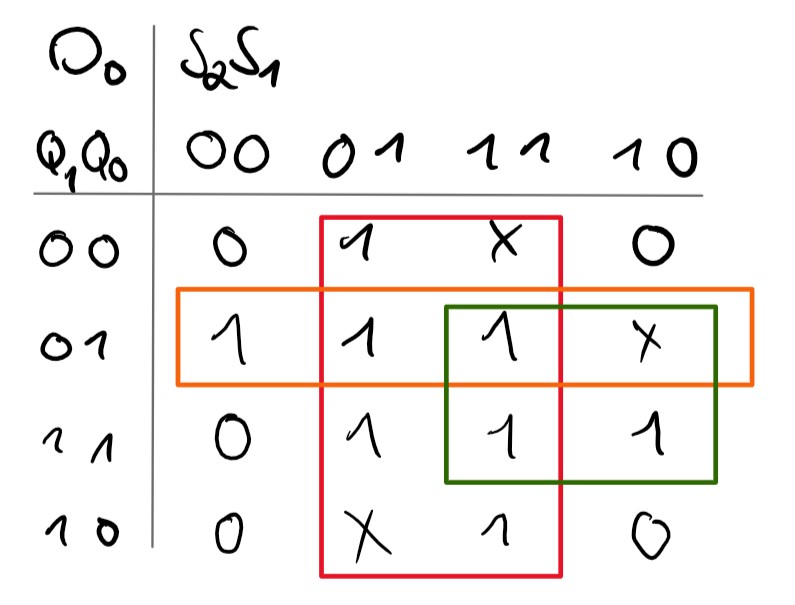
\includegraphics[width=1\textwidth]{usn1.jpg}
            \label{tab:3}    
    \end{minipage}\hfill%
    \begin{minipage}{0.5\textwidth}
        \captionof{table}{KV-Tafel für \(D_1\)}
        \label{tab:4}
        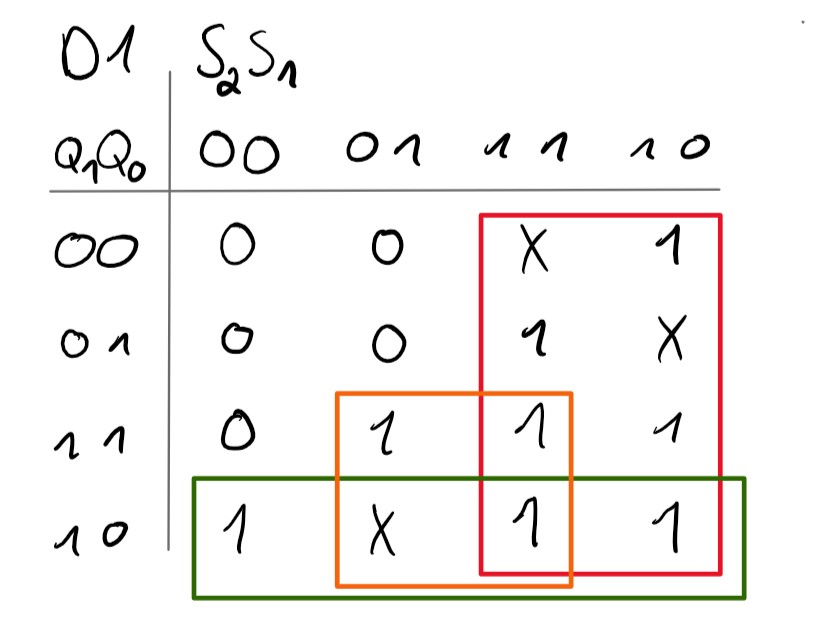
\includegraphics[width=1\textwidth]{usn2.jpg}
    \end{minipage}

    Für \(D_0\) erhält man nach Umformen der disjunktiven Minimalform in Full-NAND:
    \begin{align*}
        D_0 =& S_1 \vee (Q_0 \wedge \overline{Q_1}) \vee (S_2 \wedge Q_0)\\
        D_0 =& \overline{ \overline{\overline{\overline{S_1} \wedge \overline{ (Q_0 \wedge \overline{Q_1}) } }} \wedge \overline{ (S_2 \wedge Q_0) }}
    \end{align*}

    Gleiches Vorgehen für \(D_1\):
    \begin{align*}
        D_1 =& S_2 \vee (\overline{Q_0} \wedge Q_1) \vee (S_1 \wedge Q_1)\\
        D_1 =& \overline{ \overline{\overline{\overline{S_2} \wedge \overline{ (\overline{Q_0} \wedge Q_1) }}} \wedge \overline{ (S_1 \wedge Q_1) }}
    \end{align*}
    
\section{Realisierung des Ausgangsschaltnetzes}
    Als Nächstes wird das Ausgangsschaltnetz in Full-NAND dargestellt. Dabei wird die Wahrheitstabelle in \ref{tab:5} aufgestellt.

    \begin{table}
        \centering
        \caption{Wahrheitstabelle des ASN}
        \label{tab:5}
        \begin{tabular}{cc|cc}\toprule
            $Q_1$   &   $Q_0$   &   $Dn$    &   $Up$\\\midrule
            0       &   0       &   1       &   1\\
            0       &   1       &   1       &   0\\
            1       &   0       &   0       &   1\\
            1       &   1       &   1       &   1\\\bottomrule
        \end{tabular}
    \end{table}

    \begin{minipage}{0.5\textwidth}
        \centering
            \captionof{table}{KV-Tafel für \(Up\)}
            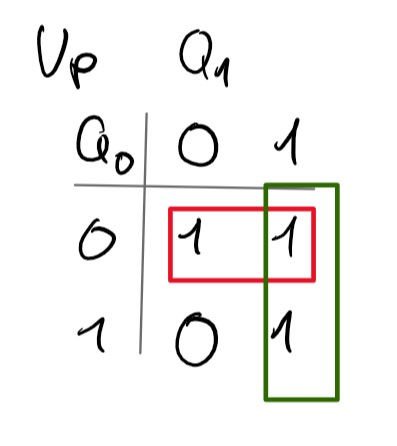
\includegraphics[width=1\textwidth]{asn1.jpg}
            \label{tab:6}    
    \end{minipage}\hfill%
    \begin{minipage}{0.5\textwidth}
        \captionof{table}{KV-Tafel für \(Dn\)}
        \label{tab:7}
        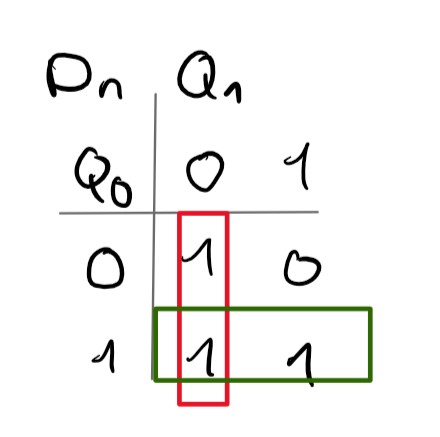
\includegraphics[width=1\textwidth]{asn2.jpg}
    \end{minipage}

    Schließlich werden auch die DMF von UP und DN durch Full-NAND realisiert.

    \begin{align*}
        Up =& \overline{Q_0} \vee Q_1\\
        UP =& \overline{Q_0 \wedge \overline{Q_1}}
    \end{align*}

    \begin{align*}
        Dn =& Q_0 \vee \overline{Q_1}\\
        Dn =& \overline{\overline{Q_0} \wedge Q_1}
    \end{align*}

\section{Vereinfachen der Full-NAND-Lösung}
    Die Terme \(\overline{\overline{Q_0} \wedge Q_1}\) und \(\overline{Q_0 \wedge \overline{Q_1}}\) des ASN kommen bereits im Übergangsschaltnetz vor. Daher können hier zwei Gatter eingespart werden. Es sind somit insgesamt 12 NAND-Gatter notwendig.

\section{Simulation der Schaltung}
    Die aufgebaute Schaltung ist Abbildung \ref{fig:1} zu entnehmen. Die Auswertung der Schaltung erzeugt die Wahrheitstabelle \ref{tab:8}. Sie stimmt mit Tabelle \ref{tab:2} und dem Zustandsdiagramm überein. Es wurde also ein korrektes Schaltungssdesign verwendet. Außerdem wurde die Anforderung an maximal 12 NAND-Gatter erfüllt.

    \begin{figure}
        \centering
        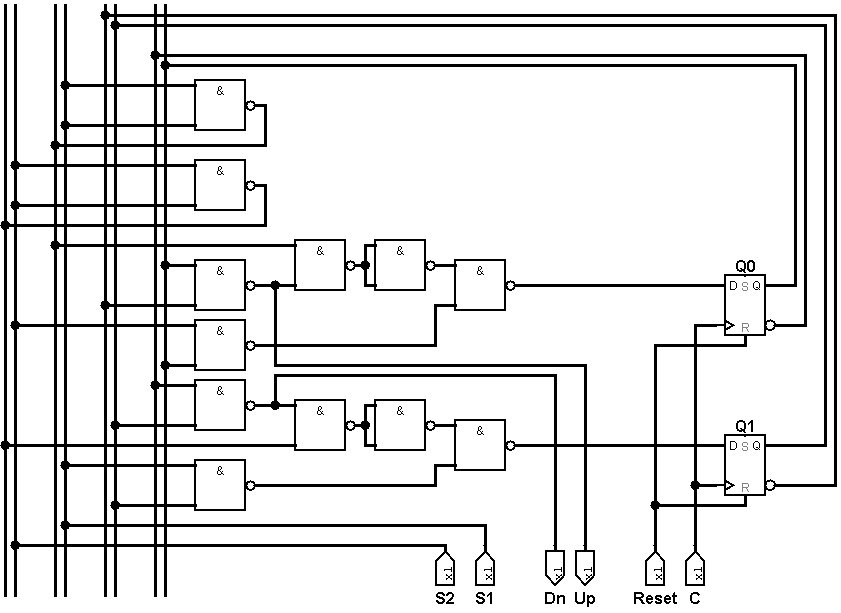
\includegraphics[width=\textwidth]{schaltung.png}
        \caption{Simulation der Schaltung}
        \label{fig:1}
    \end{figure}

    \begin{table}
        \centering
        \caption{Wahrheitstabelle der simulierten Schaltung}
        \label{tab:8}
        \begin{tabular}{cccc|cc}\toprule
            $S_2$   &   $S_1$   &   $Q_1$   &   $Q_0$   &   $Dn$    &   $Up$\\\midrule
            0       &   0       &   0       &   0       &   1       &   1\\
            0       &   1       &   0       &   0       &   1       &   0\\
            0       &   1       &   0       &   1       &   1       &   0\\
            0       &   0       &   0       &   1       &   1       &   0\\
            1       &   1       &   0       &   1       &   1       &   1\\
            1       &   1       &   1       &   1       &   1       &   1\\
            1       &   0       &   1       &   1       &   1       &   1\\
            0       &   1       &   1       &   1       &   1       &   1\\
            0       &   0       &   1       &   1       &   1       &   1\\\midrule
            0       &   0       &   0       &   0       &   1       &   1\\
            1       &   0       &   0       &   0       &   0       &   1\\
            1       &   0       &   1       &   0       &   0       &   1\\
            0       &   0       &   1       &   0       &   0       &   1\\
            1       &   1       &   1       &   0       &   1       &   1\\
            1       &   1       &   1       &   1       &   1       &   1\\
            0       &   1       &   1       &   1       &   1       &   1\\
            0       &   1       &   1       &   0       &   1       &   1\\
            0       &   0       &   1       &   1       &   1       &   1\\\bottomrule
        \end{tabular}
    \end{table}

\end{document}